\documentclass[12pt]{article}

\usepackage[utf8]{inputenc}
\usepackage[T1]{fontenc}
\usepackage{amsmath}
\usepackage{amssymb}
\usepackage{graphicx}
\usepackage{booktabs}
\usepackage{hyperref}
\usepackage[round]{natbib}
\usepackage[margin=1in]{geometry}
\usepackage{enumitem}
\usepackage{tikz}
\usetikzlibrary{positioning, arrows.meta, fit, backgrounds, calc}

\title{Analogic Appropriation: Children's Participatory Character Combat as Cross-Culturally Recurrent Play Across Three Media Eras}

\author{Jiyeon Yoon\\
Independent Researcher\\
\texttt{wantcongz@gmail.com}}

\date{Preprint --- Submitted to MediArXiv\\March 2026}

\begin{document}

\maketitle

\begin{abstract}
Children in culturally distinct settings independently create characters on paper and pit them against peers' creations in rule-governed combat. We propose ``analogic appropriation'' --- grounded in Corsaro's interpretive reproduction, Caillois's play typology, and de Certeau's tactics --- to explain this cross-culturally recurrent phenomenon. Digital documentary analysis across seven countries (five core cases and two boundary cases) and five decades reveals three eras: analog appropriation (1970s--2000s), in which Korean notebook RPGs, American Pencil Wars, and Indonesian Perang-perangan reproduced dominant media interfaces on paper; digital democratization (2010s--2020s), exemplified by child-created Roblox games; and AI-mediated folk art (2025--), exemplified by Italian brainrot. A recurrent core --- participatory character creation, agonistic structure, peer sharing --- persists across eras and settings. We address the Galton Problem of independent invention versus diffusion, identify boundary conditions through counterexamples, and outline a planned eight-country survey to test the framework empirically.

\medskip
\noindent\textbf{Keywords:} analogic appropriation, children's play, cross-cultural, interpretive reproduction, digital folklore, participatory culture
\end{abstract}

%----------------------------------------------------------------------
\section{Introduction}

\subsection{A Cross-Cultural Puzzle}

Ask any Korean adult born in the 1990s about ``gonghchaek geim'' (notebook games), and a wave of nostalgia is likely to follow. They will describe drawing characters with hit points and attack statistics in school notebooks, constructing virtual shops and hunting grounds on lined paper, and battling friends' characters through improvised damage formulas --- sometimes calculated with actual calculators brought to school \citep{namuwiki}. Now ask an American adult born in the 1970s about ``Pencil Wars.'' They will describe folding paper in half, drawing tanks on each side, flicking pencils to shoot lines across the crease, and destroying opponents' units when the line crosses a drawn figure \citep{straightdope2016}. Ask a Turkish adult about ``Kareli Defterde Imparatorluk Oyunu'' --- the grid-paper empire game --- and they will recall eraser dice, territorial conquest on graph paper, and elaborate military hierarchies sketched during class \citep{eksisozluk}. Ask an Indonesian about the fold-and-dot game played on school benches, and they will describe what they call ``Perang-perangan'' --- a paper battle whose mechanics are functionally identical to the American version, yet whose players have never heard of one another.

These groups are separated by oceans, decades, and entirely different cultural contexts. Yet the underlying structure is strikingly similar: \emph{create characters or units on paper, establish rules for combat, fight with peers}. This recurrence across culturally distinct settings constitutes a theoretical puzzle that existing scholarship has not adequately addressed.

This paper asks three questions:

\medskip
\noindent\textbf{RQ1:} How widespread is paper-based character combat play, and what patterns of independent emergence versus diffusion can be identified across culturally distinct settings?

\medskip
\noindent\textbf{RQ2:} How does the specific form of this play relate to the dominant media interfaces available to children in each era?

\medskip
\noindent\textbf{RQ3:} What structural elements persist across analog, digital, and AI-mediated manifestations of participatory character creation?

\subsection{The Theoretical Gap}

Despite rich traditions of research on children's play \citep{opie1969,edwards2000,burn2014}, digital folk culture \citep{blank2012,owens2025}, and participatory media \citep{jenkins2006,ito2010}, no existing framework captures the specific phenomenon documented here: children's sustained, rule-governed creative combat play that (a) recurs across culturally distinct settings, (b) systematically appropriates dominant media interfaces onto available material substrates, and (c) persists across successive media eras in structurally recognizable form. \citet{burn2014} made foundational contributions by documenting how children's playground games incorporate new media elements, but their analysis centered on the United Kingdom and did not trace the cross-cultural or diachronic scope that our documentary evidence reveals. The present paper addresses this gap by proposing a theoretical framework --- grounded in interpretive reproduction, play typology, and the tactics of everyday practice --- and illustrating it through cross-cultural documentary analysis.

\subsection{Contribution}

This paper makes three contributions. First, it offers the first systematic cross-cultural documentation of paper-based character combat play, with illustrative evidence from five core settings (Korea, the United States, Turkey, Indonesia, and the Philippines), two boundary cases that illuminate the phenomenon's limits (Russia and India), and a theoretically significant discussion of Japan's apparent absence. Second, it proposes a theoretical framework --- ``analogic appropriation'' --- that synthesizes Corsaro's interpretive reproduction with Caillois's agon and mimicry, de Certeau's tactics, and Vygotsky's developmental rehearsal to explain why this play recurs and why its form tracks dominant media. Third, it traces this practice across three media eras, from analog paper through digital platforms to AI-generated imagery, identifying both structural continuities and meaningful discontinuities.

%----------------------------------------------------------------------
\section{Theoretical Framework}

\subsection{Interpretive Reproduction: Children as Creative Appropriators}

The central theoretical resource for this paper is \citeauthor{corsaro2005}'s (\citeyear{corsaro2005}) concept of \emph{interpretive reproduction}. Against developmental models that treat children as passive recipients of adult culture, Corsaro demonstrated that children creatively appropriate elements of the adult world to produce and participate in their own peer cultures. This appropriation is ``interpretive'' because children do not simply imitate adult practices but transform them in accordance with peer-culture concerns --- status, fairness, imaginative elaboration, and collective enjoyment.

We argue that paper-based character combat play is a paradigmatic case of interpretive reproduction. When Korean children of the early 2000s drew MapleStory-style stat windows in their notebooks, they were not merely imitating a video game. They were creatively appropriating the affordances of a digital interface --- character statistics, inventory management, quest progression --- and transplanting them onto the material substrate available in the classroom: paper, pencils, and the social infrastructure of the peer group. The resulting ``notebook RPG'' was neither a faithful copy of MapleStory nor an independent invention unrelated to it; it was an interpretive reproduction that served peer-culture functions (status negotiation through the operator role, collective world-building, agonistic engagement) that the original digital game could not provide in the same way.

\subsection{Agon and Mimicry: Caillois's Play Classification}

\citet{caillois1961} classified play along two axes that prove directly applicable to our phenomenon. \emph{Agon} (competition) describes play governed by formal equality of conditions in which participants seek to establish superiority --- the combat dimension of paper character play, from Korean notebook RPG damage calculations to American pencil-flicking wars. \emph{Mimicry} (simulation/role-play) describes play in which participants adopt illusory identities --- the character creation dimension, in which children invest imaginative labor in constructing personas with names, attributes, and visual identities.

Paper combat play fuses agon and mimicry in a distinctive configuration. The competitive dimension provides the stakes (winning, losing, the destruction or survival of one's character), while the mimicry dimension provides the affective investment (identification with one's created character, narrative elaboration of combat outcomes). This fusion is not trivial; Caillois himself noted that agon and mimicry can combine but did not systematically analyze child-initiated instances of this combination. We propose that the recurrence of this agon-mimicry fusion across cultural settings reflects a deep structural affordance of play itself --- one that children discover independently when given minimal material resources (paper, writing implements) and the social context of a peer group.

\citeauthor{huizinga1938}'s (\citeyear{huizinga1938}) concept of the \emph{magic circle} --- the bounded spatial and temporal frame within which play operates under its own rules --- further illuminates why the classroom notebook, the folded sheet of paper, or the digital platform functions as a play space. The notebook page becomes a magic circle: within its bounds, drawn characters possess hit points that matter, shops sell imaginary goods for imaginary currency, and the operator's authority is real. The magic circle concept helps explain why this play feels intensely meaningful to its participants despite --- or precisely because of --- its separation from the ``real'' world of adult concerns.

\subsection{Tactics and Poaching: de Certeau and Children's Appropriation}

\citet{decerteau1984} distinguished between \emph{strategies} --- the operations of those who possess institutional power and can define spaces --- and \emph{tactics} --- the improvisational maneuvers of those who operate within spaces defined by others. Children in classrooms are quintessential tactical actors: they lack the power to define the institutional space (the school, the curriculum, the schedule) but constantly find ways to repurpose that space for their own ends.

Paper combat play is a tactical appropriation in de Certeau's precise sense. The notebook is a curricular object repurposed for play. The classroom is an institutional space temporarily converted into an arena. Most significantly, the digital game --- an adult-produced commercial product that children cannot always access (due to cost, parental restrictions, school hours, or limited PC room time in the Korean context) --- is ``poached'' and reconstructed on paper. Korean children who drew MapleStory interfaces in their notebooks were engaging in what de Certeau would recognize as tactical consumption: unable to control access to the digital game, they reproduced its essential features using the materials at hand. This framing avoids the implicit technological determinism of treating children as mere recipients of media influence and instead foregrounds their creative agency within structural constraints.

\subsection{Developmental Rehearsal: Vygotsky and the Zone of Proximal Development}

\citeauthor{vygotsky1978}'s (\citeyear{vygotsky1978}) zone of proximal development (ZPD) offers a developmental lens on the operator role in paper combat play. In the Korean notebook RPG, the ``unjyeongja'' (operator/game master) designed game systems, balanced economies, adjudicated disputes, and managed player experience --- functions that in the digital world require programming skill, design knowledge, and project management capacity that most elementary school children do not yet possess. The notebook medium provided a scaffold within which children could rehearse these complex cognitive and social operations at a developmentally appropriate level of abstraction. The operator role, we suggest, functioned as a ZPD space: children performing game design with paper and pencil were practicing, in simplified form, the same design thinking that would later be exercised in Roblox Studio or game development engines.

\citet{kafai2016} extended this developmental logic through the lens of \emph{constructionist gaming}, arguing that children learn most deeply when they make games rather than merely play them. The notebook RPG operator was a constructionist game designer avant la lettre --- building systems, testing them with peers, iterating in response to feedback --- using the humblest possible technology.

\subsection{Analogic Appropriation: An Integrative Concept}

We propose \emph{analogic appropriation} as an integrative term for the phenomenon documented in this paper. The term captures three dimensions simultaneously. First, ``analogic'' references the analog material substrate (paper, pencil) onto which digital affordances are transposed --- a process loosely analogous to what \citet{bolter1999} theorized as remediation, though operating in the reverse direction (from digital to analog) and driven by children's tactical needs rather than media-industry logics. We invoke remediation here as a metaphorical resource rather than a strict theoretical application, since Bolter and Grusin's framework was developed to describe how new media refashion prior media, not how children reconstruct inaccessible digital media on paper. Second, ``analogic'' invokes analogical reasoning --- the cognitive process by which children identify structural correspondences between a digital game and a paper notebook and exploit those correspondences to create playable systems. Third, ``appropriation'' connects to both Corsaro's interpretive reproduction (children appropriating adult culture for peer-culture purposes) and de Certeau's tactics (subordinate actors poaching from dominant cultural forms). We retain the term across all three eras because the second dimension --- analogical reasoning --- persists even when the analog substrate does not: the Roblox developer who structures a game around stat-based combat is drawing structural correspondences from the same MMORPG grammar that the notebook RPG operator drew, and the brainrot creator who assigns power levels to AI-generated characters is performing the same analogical mapping onto a new substrate.

We define the \emph{dominant interface effect} as the tendency for children's analogic appropriation to gravitate toward whichever media interface they engage with most intensely, reproducing its formal characteristics (visual layout, interaction grammar, rule systems) on whatever substrate is available. This effect is bounded by several scope conditions: it requires (a) sustained engagement with a dominant medium sufficiently complex to offer appropriable structures, (b) a gap between the child's expressive intent and the medium's native affordances --- whether that gap is one of physical access (Era~1: children who cannot reach the PC room), technical skill (Era~2: children who lack programming fluency), or creative control (Era~3: children who can generate images but not author the narrative and competitive frameworks that give those images meaning within peer culture), and (c) a peer group with shared media knowledge that can serve as an interpretive community for the appropriated forms.

\subsection{A Direct Predecessor: Burn and Richards (2014)}

Our framework builds on \citeauthor{burn2014}'s (\citeyear{burn2014}) \emph{Children's Games in the New Media Age}, which documented how British children wove video game characters and mechanics into playground games. Our contribution extends theirs in three respects: (a) cross-cultural scope across seven countries rather than one; (b) foregrounding material substrate as an analytically significant variable (paper versus playground versus platform versus AI); and (c) diachronic analysis across three media eras rather than a single historical moment.

\subsection{Self-Critique: The Rhetoric of Progress}

\citet{suttonsmith1997} cautioned that scholarship on children's play is pervaded by what he termed ``rhetorics'' --- implicit ideological frameworks that shape how researchers interpret play phenomena. The \emph{rhetoric of progress} treats play as preparation for adult competence, emphasizing its developmental benefits and cognitive scaffolding functions. We acknowledge that our framework --- particularly the invocation of Vygotsky's ZPD and Kafai's constructionism --- risks reproducing this rhetoric by framing paper combat play primarily as developmental rehearsal for ``real'' (i.e., adult-valued) game design.

We therefore register an explicit caveat: paper combat play may be valuable to children for reasons entirely unrelated to adult-defined developmental outcomes. It may be valued for the sheer pleasure of agonistic engagement, for the aesthetic satisfaction of character creation, for the social bonding of shared secret worlds, or for the subversive pleasure of repurposing school materials against institutional purposes. A complete account of the phenomenon must hold these possibilities alongside developmental interpretations, resisting the temptation to justify children's play solely in terms of its instrumentality for adult-valued skills.

%----------------------------------------------------------------------
\section{Methodology: Digital Documentary Analysis}

\subsection{Approach and Epistemological Status}

This paper employs digital documentary analysis of publicly available online sources to construct an illustrative cross-cultural account of paper-based character combat play. We draw on what \citet{blank2012} termed the study of ``folk culture in the digital age'' --- attending to the ways in which vernacular cultural practices leave traces in online environments that can serve as evidence for cultural analysis. Our approach is explicitly illustrative rather than exhaustive: we do not claim to have surveyed all instances of this play worldwide, but rather to have assembled sufficient cross-cultural evidence to motivate and illustrate a theoretical framework.

We distinguish four source types --- wiki documentation (Namuwiki), student-collected folklore data (USC Digital Folklore Archives), online forum testimonies (Straight Dope, Hacker News, Eksi Sozluk), and journalistic/meme-documentation sources (Know Your Meme, ABC News) --- each treated with appropriate epistemic caution (see Supplementary Materials S3).

\subsection{Limitations of Method}

Digital documentary analysis cannot establish prevalence, representativeness, or causal relationships. The evidence assembled here is subject to Anglophone and Koreanophone bias (cultures with rich online documentation are overrepresented), survivorship bias (practices that left digital traces are visible while others are not), and retrospective reconstruction (adults remembering childhood play may narrativize it in ways that emphasize coherence). We present this evidence as sufficient to motivate a theoretical framework and identify a cross-culturally recurrent pattern, not as proof of universality. As this study analyzes publicly available online content and does not involve human participants, institutional ethics review was not required.

%----------------------------------------------------------------------
\section{Three Eras of Analogic Appropriation: Cross-Cultural Evidence and Analysis}

Table~\ref{tab:evidence} summarizes the cross-cultural evidence across all three eras.

\begin{table}[htbp]
\centering
\caption{Summary of Cross-Cultural Evidence Across Three Eras}
\label{tab:evidence}
\small
\begin{tabular}{@{}p{1.4cm}p{1.2cm}p{1.8cm}p{2.0cm}p{2.0cm}p{1.6cm}p{1.8cm}p{1.2cm}@{}}
\toprule
Country & Era & Local Name & Core Mechanic & Dominant Media Context & Primary Source Type & Evidence Level & Case Status \\
\midrule
Korea & 1 (1970s--2000s) & Gonghchaek geim (notebook RPG) & Stat-based character creation, operator-managed RPG on paper & MMORPGs (MapleStory, Ragnarok Online, Baram) & Wiki documentation (Namuwiki) & Strong (detailed community documentation) & Core \\
\addlinespace
USA & 1 (1970s--1990s) & Pencil Wars / Tanks / Paper Battle & Fold-and-dot transfer; pencil-flick attack lines & Tabletop wargaming, TV action, early arcade & Folklore archives (USC), forum testimonies & Moderate (multiple independent sources) & Core \\
\addlinespace
Turkey & 1 (est.\ 1990s--2000s) & Kareli Defterde Imparatorluk Oyunu & Grid-paper territorial conquest, eraser dice & Board gaming, tabletop RPG, Ottoman history curricula & Forum testimonies (Eksi Sozluk) & Moderate (multiple testimonies) & Core \\
\addlinespace
Indonesia & 1 (est.\ 1990s--2000s) & Perang-perangan & Fold-and-dot transfer (identical to US Paper Battle) & Local media environment & Journalistic sources & Moderate (media documentation) & Core \\
\addlinespace
Philippines & 1 (est.\ 1990s--2000s) & Spaceship & Fold-and-dot transfer (spacecraft variant) & Local media environment & Journalistic sources & Low-moderate (limited documentation) & Core \\
\addlinespace
Russia/ E.~Europe & 1 (Soviet era--2000s) & Tochki, Klopy, Amoeba & Territorial enclosure, abstract strategy on graph paper & Chess/abstract strategy tradition & Forum testimonies (Hacker News) & Moderate & Boundary (lacks mimicry/ character creation) \\
\addlinespace
India & 1 (est.\ 1990s--2010s) & Pen Fight & Flicking pens off desk edges & School implements culture & Folklore archives (USC), journalism & Moderate (national championship documented) & Boundary (lacks character creation) \\
\addlinespace
Japan & 1--3 & (Thin Era~1 evidence; strong Era~3 adoption) & Era~1: Limited ``Tanks'' in cross-cultural context; Era~3: brainrot adoption & RPG Maker (1992), RPGs, shonen manga; AI tools (2025) & Folklore archives; industry reports (KADOKAWA) & Low (Era~1) / Strong (Era~3) & Theoretically instructive absence \\
\addlinespace
Global (Era~2) & 2 (2010s--2020s) & Roblox/ Minecraft/ Fortnite Creative & Platform-native game creation by children & Digital creation platforms & Industry data (Naavik, Versework) & Strong (quantitative platform data) & Structural continuity case \\
\addlinespace
Global (Era~3) & 3 (2025--) & Italian brainrot & AI-generated characters with pseudo-Italian names, power-level battles & AI image generation, TikTok/ YouTube & Meme documentation, journalism, industry reports & Strong (real-time documentation) & Core \\
\bottomrule
\end{tabular}
\end{table}

\subsection{Era 1: Analog Appropriation (1970s--2000s)}

\subsubsection{Korea: Notebook RPGs (gonghchaek geim)}

The most richly documented case comes from South Korea, where ``gonghchaek geim'' (notebook games) were widespread among children born approximately 1985--2000 \citep{namuwiki}. The notebook RPG involved character creation with numerical statistics (HP, attack power, defense, speed); world-building by a designated ``unjyeongja'' (operator) who drew shops, hunting grounds, and quest locations; an economic system with in-game currency; combat resolution through damage formulas; and social dynamics in which the operator could grant favors, creating informal power hierarchies. Critically, the visual language directly mirrored contemporary Korean MMORPGs --- MapleStory (2003), Ragnarok Online (2002), and Baram (1996). Children replicated stat windows, inventory screens, and shop interfaces as visual copies drawn on paper --- a clear instance of analogic appropriation: tactically reconstructing an inaccessible digital interface on an available material substrate.

\subsubsection{Other Core Cases}

\textbf{United States} (1970s--1990s): American children developed ``Tanks'' (flicking pencils to draw attack lines; documented at the USC Digital Folklore Archives~\citep{uscfolklore} across Japanese and American students in Okinawa) and ``Paper Battle'' / ``Pencil Wars'' (fold-and-dot-transfer mechanics; \citealp{instructables}). The dominant media environment --- tabletop wargaming, television action, early arcade --- shaped these variants toward physical mechanics over statistical abstraction, consistent with the dominant interface effect.

\textbf{Turkey} (1990s--2000s): ``Kareli Defterde Imparatorluk Oyunu'' (grid-paper empire war), documented on Eksi Sozluk, featured territorial conquest on graph paper with eraser dice --- suggesting appropriation from board gaming and tabletop RPG traditions, with military-imperial theming possibly reflecting Ottoman history curricula.

\textbf{Indonesia} (1990s--2000s): ``Perang-perangan'' uses fold-and-dot-transfer mechanics functionally identical to American Paper Battle, yet no transmission pathway connects them --- suggestive evidence for independent emergence from shared material constraints.

\textbf{Philippines} (1990s--2000s): ``Spaceship'' parallels both American and Indonesian fold-and-dot mechanics with spacecraft variants. The geographic distribution raises the possibility of diffusion through maritime contact, though evidence is insufficient.

\subsubsection{Boundary Cases}

\textbf{Russia/Eastern Europe}: Soviet pen-and-paper strategy games --- ``Tochki'' (territorial enclosure), ``Klopy'' (four-player diplomacy on graph paper) --- share agonistic and peer-sharing dimensions but lack mimicry-driven character creation, reflecting the chess and abstract strategy tradition rather than digital media \citep{hackernews2017}. \textbf{India}: ``Pen Fight'' (flicking pens off desk edges) achieved national championship status spanning 21 states, sharing the school-implements-agon-peers structure while lacking character creation --- defining the boundary of our focal phenomenon.

\subsection{Era 2: Digital Democratization (2010s--2020s)}

The second era is marked by the availability of digital creation tools accessible to children. Roblox (2006, mass adoption in the 2010s), Minecraft (2011), and Fortnite Creative/UEFN (2018/2023) provided children with the means to realize the creative-agonistic impulse \emph{within} the dominant medium itself rather than transposing it onto paper. The scale of this shift is now quantifiable: Roblox reported 144 million daily active users and \$6.8 billion in annual bookings for 2025, with creators receiving over \$1.5 billion in revenue share --- constituting two-thirds of the non-China gaming industry's net consumer spending growth \citep{naavik2026}.

A terminological caveat is necessary. Era~2 represents \emph{structural continuity} with Era~1 rather than analogic appropriation in the strict sense. In \citeauthor{decerteau1984}'s (\citeyear{decerteau1984}) terms, tactics involve repurposing tools against or beyond their intended function; Roblox Studio, however, is explicitly designed for children to create games --- using it as intended is \emph{use}, not tactical appropriation. We retain Era~2 in our framework because the underlying creative-agonistic-peer-sharing configuration persists, but we distinguish it from Era~1's genuine appropriation (reconstructing digital interfaces on unauthorized substrates) and Era~3's reverse appropriation (using AI tools to generate characters in ways not anticipated by tool designers). The concept of ``analogic appropriation'' applies most strictly to Era~1; Era~2 demonstrates the \emph{persistence of the impulse} when access constraints are removed, while Era~3 demonstrates its \emph{re-emergence} in a new technological context.

The structural continuity between the notebook RPG operator and the Roblox developer is striking (see also \citealp{cds2025}, for Indonesian children's Roblox use). Both design game systems, establish rules, build worlds, manage player experiences, and derive social status from their creative-managerial role. The Korean game ``Sols RNG,'' created by a development team with an average age of 17.8, crossed 1.3 billion visits on Roblox \citep{versework2025}. In Corsaro's terms, these young developers are performing interpretive reproduction of adult game-industry practices, appropriating professional game design conventions for peer-culture purposes --- precisely as the notebook RPG operator did, but now using the same digital substrate that was previously appropriated only in analog form.

What changes in Era~2 is the scope of both creation and sharing. The notebook RPG's magic circle was bounded by the physical classroom; the Roblox experience's magic circle extends globally. The operator's authority was personal and immediate; the developer's authority is mediated by platform architecture. Caillois's agon remains central (competitive gameplay is the dominant genre on Roblox), as does mimicry (character creation and customization are core to platform engagement). But the material substrate has shifted from paper to code, and with it the developmental rehearsal function: where notebook RPG operation rehearsed game design thinking, Roblox development rehearses programming, UI design, and digital project management --- skills that \citet{kafai2016} argue constitute the core of constructionist gaming education.

\subsection{Era 3: AI-Mediated Folk Art (2025--)}

The third era began in early 2025 with the explosion of ``Italian brainrot'' --- a participatory meme culture in which children and teenagers use AI image generation tools to create bizarre characters, assign them pseudo-Italian names, and pit them against each other in imagined battles shared via TikTok and YouTube. ``Tung Tung Tung Sahur,'' the most viral character, was posted on February 28, 2025, and accumulated over 42.5 million views within days \citep{kym2025}. The character spawned hundreds of derivative characters created by children worldwide.

Animator Fabian Mosele characterized Italian brainrot as ``internet folklore --- a grassroots, participatory universe that big studios have no control over'' \citep{abcnews2025}, aligning with theorizations of folklore in algorithmic environments where platform logics reshape but do not eliminate vernacular creativity \citep{flinterud2023}. \citet{barchiesi2025} offered a more theoretically developed reading, describing Italian brainrot as ``fragments of a European anime culture in the making'' --- characters in search of a story, following the opposite trajectory from narrative-first traditions like Tintin. We concur with these characterizations and further argue that Italian brainrot represents the latest manifestation of the analogic appropriation tradition --- now operating in the reverse direction. Where Era~1 children appropriated digital interfaces \emph{onto} paper, Era~3 children appropriate the act of character creation \emph{through} AI, bypassing both manual drawing and programming. The dominant interface effect is again visible: the specific form of character creation (prompt-based AI image generation) mirrors the dominant tool environment of 2025, just as notebook RPG stat windows mirrored the dominant game interfaces of 2003.

The speed at which Era~3 has scaled dwarfs all precedents. On Roblox, the game \emph{Steal a Brainrot} --- released May 2025 --- accumulated over 60 billion visits and reached a peak of 25.4 million concurrent users, the highest in Roblox history \citep{pocketgamer2025}. The Italian company Skifidol acquired formal IP rights and launched a Panini trading-card game and sticker album; Spin Master secured exclusive North American distribution \citep{licenseglobal2026}; Epic Games licensed the IP for Fortnite Creative (2025). In Japan, Kadokawa Game Linkage announced two brainrot encyclopedias for children, scheduled for April 2026 --- responding to survey data showing ``Italian brainrot'' as the top buzzword among elementary school girls \citep{automaton2026}. What began as grassroots folk art in January 2025 had, within twelve months, become a multi-platform commercial IP --- a trajectory that compresses into a single year a commercialization arc that took decades for comparable folk-to-industry phenomena. The participatory spectacle dynamics visible in brainrot parallel what \citet{melo2026} documented as ``memetic performance'' in the Minecraft Movie phenomenon --- ritualized agonistic-creation-peer-sharing cycles amplified by platform affordances.

Italian brainrot reproduces the core structure of paper combat play: participatory character creation (anyone can generate a new character using free AI tools), agonistic framing (characters are positioned in opposition --- ``Bombardiro Crocodilo vs.\ Tung Tung Tung Sahur''), and peer sharing (characters are circulated via social media for validation and elaboration). The platform itself cultivates this dynamic: \citet{divon2025} argue that TikTok's ``playability'' functions not merely as a creative prompt but as a structural affordance through which users produce, interpret, and disseminate content --- a logic that extends the magic circle from the classroom notebook to the algorithmic feed. What has changed is the entry barrier (from pencil skill to text prompts), the sharing range (from classroom to global), and the persistence (from notebook lifespans to meme lifecycles). The fundamental agon-mimicry fusion identified by Caillois's framework persists --- and, as recent qualitative research confirms, participants experience brainrot not as passive consumption but as active agency recovery within an extractive attention economy \citep{gotzfried2026}.

\subsection{The Recurrent Core: Agonistic Creation and Peer Sharing}

Across all three eras and the documented cultural settings, we identify a recurrent configuration that we term the \emph{agonistic creation core} (see Figure~\ref{fig:cross-era} for a visual summary of what persists and what changes across eras):

\begin{enumerate}[leftmargin=*]
    \item \textbf{Participatory character creation (mimicry):} The child \emph{creates} --- not merely selects --- a character, unit, or entity with personal investment. This act of creation engages what \citet{caillois1961} termed mimicry: the child imaginatively inhabits or identifies with their creation.

    \item \textbf{Agonistic structure (agon):} The created entities are placed in opposition --- fighting, competing, conquering --- under some form of rule governance, however minimal. Following Caillois, we use ``agonistic structure'' rather than ``combat'' to encompass the range of competitive forms documented: statistical damage calculation (Korea), physical flicking (USA), territorial conquest (Turkey), and imagined power hierarchies (Italian brainrot).

    \item \textbf{Peer sharing:} The creation and competition are performed \emph{with and for} peers, constituting what \citet{corsaro2005} would recognize as peer-culture production. The social dimension is not incidental but constitutive: solitary character drawing is art; solitary combat is physical play; it is the combination within a peer-cultural frame that produces the distinctive phenomenon.
\end{enumerate}

\begin{figure*}[htbp]
\centering
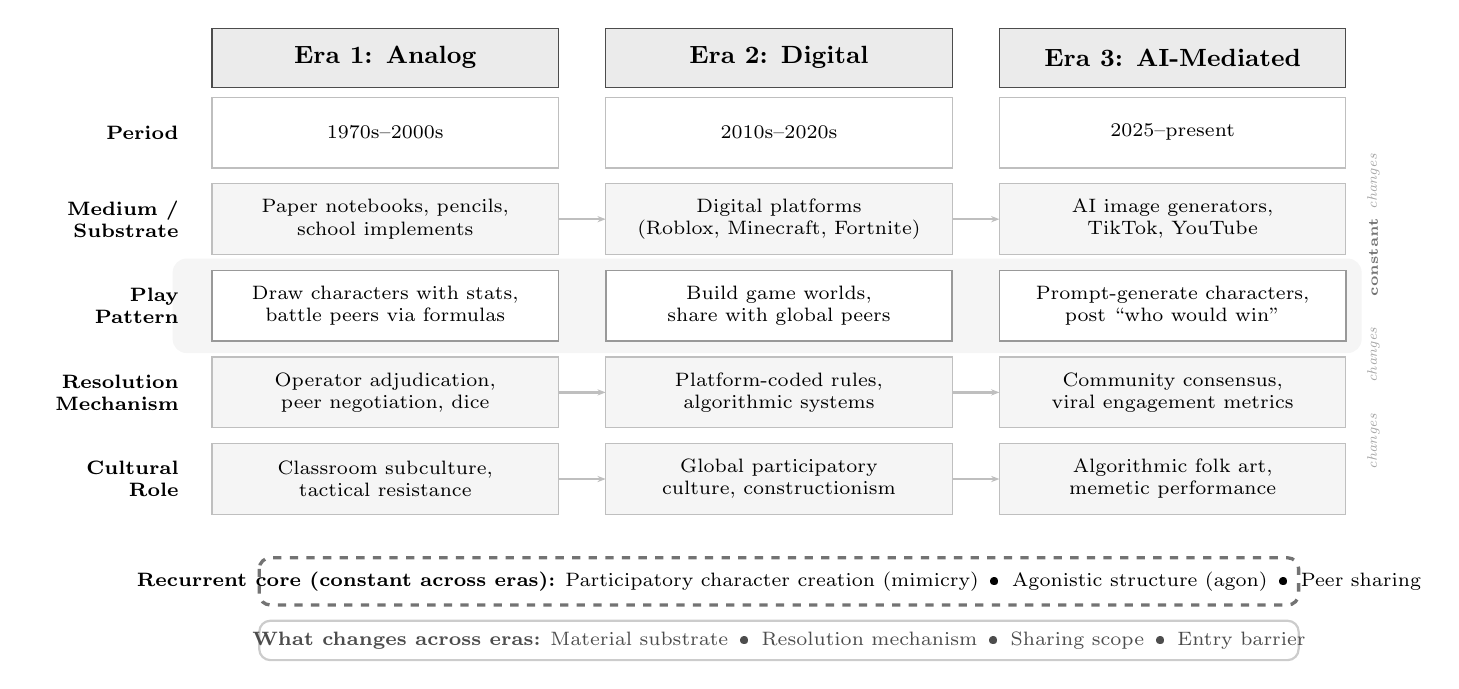
\begin{tikzpicture}[
    % Style definitions
    era/.style={
        rectangle, draw=black!70, fill=black!8,
        minimum width=4.4cm, minimum height=0.75cm,
        font=\bfseries\small, align=center
    },
    cell/.style={
        rectangle, draw=black!25, fill=white,
        minimum width=4.4cm, minimum height=0.9cm,
        font=\scriptsize, align=center, text width=4.0cm
    },
    changecell/.style={
        cell, fill=gray!8
    },
    constcell/.style={
        cell, fill=white, draw=black!40, line width=0.6pt
    },
    rowlabel/.style={
        font=\scriptsize\bfseries, align=right, text width=1.8cm,
        anchor=east
    },
    changearrow/.style={
        -{Stealth[length=3pt]}, gray!50, line width=0.8pt
    },
    changelabel/.style={
        font=\tiny\itshape, text=gray!70
    },
]

% Column positions
\def\colA{0}
\def\colB{5.0}
\def\colC{10.0}

% Row positions (top to bottom)
\def\rowTitle{0}
\def\rowPeriod{-0.95}
\def\rowMedium{-2.05}
\def\rowPattern{-3.15}
\def\rowResolution{-4.25}
\def\rowRole{-5.35}

% === Era headers ===
\node[era] at (\colA, \rowTitle) {Era 1: Analog};
\node[era] at (\colB, \rowTitle) {Era 2: Digital};
\node[era] at (\colC, \rowTitle) {Era 3: AI-Mediated};

% === Period row ===
\node[rowlabel] at (-2.5, \rowPeriod) {Period};
\node[cell] at (\colA, \rowPeriod) {1970s--2000s};
\node[cell] at (\colB, \rowPeriod) {2010s--2020s};
\node[cell] at (\colC, \rowPeriod) {2025--present};

% === Medium / Substrate row (CHANGES) ===
\node[rowlabel] at (-2.5, \rowMedium) {Medium /\\Substrate};
\node[changecell] at (\colA, \rowMedium) {Paper notebooks, pencils,\\school implements};
\node[changecell] at (\colB, \rowMedium) {Digital platforms\\(Roblox, Minecraft, Fortnite)};
\node[changecell] at (\colC, \rowMedium) {AI image generators,\\TikTok, YouTube};

% === Play Pattern row (CONSTANT --- the recurrent core) ===
\node[rowlabel] at (-2.5, \rowPattern) {Play\\Pattern};
\node[constcell] at (\colA, \rowPattern) {Draw characters with stats,\\battle peers via formulas};
\node[constcell] at (\colB, \rowPattern) {Build game worlds,\\share with global peers};
\node[constcell] at (\colC, \rowPattern) {Prompt-generate characters,\\post ``who would win''};

% === Resolution Mechanism row (CHANGES) ===
\node[rowlabel] at (-2.5, \rowResolution) {Resolution\\Mechanism};
\node[changecell] at (\colA, \rowResolution) {Operator adjudication,\\peer negotiation, dice};
\node[changecell] at (\colB, \rowResolution) {Platform-coded rules,\\algorithmic systems};
\node[changecell] at (\colC, \rowResolution) {Community consensus,\\viral engagement metrics};

% === Cultural Role row (CHANGES) ===
\node[rowlabel] at (-2.5, \rowRole) {Cultural\\Role};
\node[changecell] at (\colA, \rowRole) {Classroom subculture,\\tactical resistance};
\node[changecell] at (\colB, \rowRole) {Global participatory\\culture, constructionism};
\node[changecell] at (\colC, \rowRole) {Algorithmic folk art,\\memetic performance};

% === Transition arrows between eras (for changing rows) ===
\foreach \r in {\rowMedium, \rowResolution, \rowRole} {
    \draw[changearrow] (\colA+2.2, \r) -- (\colB-2.2, \r);
    \draw[changearrow] (\colB+2.2, \r) -- (\colC-2.2, \r);
}

% === CONSTANT band highlighting the Play Pattern row ===
\begin{scope}[on background layer]
    \fill[black!4, rounded corners=5pt]
        (-2.7, \rowPattern+0.6) rectangle (\colC+2.4, \rowPattern-0.6);
\end{scope}

% === Recurrent Core annotation (below the grid) ===
\draw[black!55, line width=1.2pt, dashed, rounded corners=4pt]
    (-1.6, -6.35) rectangle (\colC+1.6, -6.95);
\node[font=\scriptsize, align=center] at (\colB, -6.65) {%
    \textbf{Recurrent core (constant across eras):}
    Participatory character creation (mimicry)
    \,\textbullet\, Agonistic structure (agon)
    \,\textbullet\, Peer sharing};

% === ``What Changes'' annotation ===
\draw[gray!40, line width=0.8pt, rounded corners=4pt]
    (-1.6, -7.15) rectangle (\colC+1.6, -7.65);
\node[font=\scriptsize, align=center, text=black!70] at (\colB, -7.4) {%
    \textbf{What changes across eras:}
    Material substrate
    \,\textbullet\, Resolution mechanism
    \,\textbullet\, Sharing scope
    \,\textbullet\, Entry barrier};

% === Side annotations for constant vs.\ changing ===
\node[changelabel, anchor=west, rotate=90] at (\colC+2.55, \rowMedium) {changes};
\node[font=\tiny\bfseries, text=black!55, anchor=west, rotate=90] at (\colC+2.55, \rowPattern) {constant};
\node[changelabel, anchor=west, rotate=90] at (\colC+2.55, \rowResolution) {changes};
\node[changelabel, anchor=west, rotate=90] at (\colC+2.55, \rowRole) {changes};

\end{tikzpicture}
\caption{Cross-era comparison framework for analogic appropriation. Each column represents one media era; rows capture the analytical dimensions. The highlighted band identifies the \emph{recurrent core} --- participatory character creation, agonistic structure, and peer sharing --- that persists across all three eras. Gray arrows mark dimensions that transform between eras (medium, resolution mechanism, cultural role), and side labels distinguish constant from changing dimensions. The dashed box below the grid summarizes the structural invariant; the solid box lists what varies.}
\label{fig:cross-era}
\end{figure*}

\subsubsection{Counterexamples and Boundary Conditions}

This recurrent core is not invariant. Counterexamples help define its boundaries. Creation without agonistic structure produces paper dolls, fashion design notebooks, and collaborative world-building --- practices that share the mimicry and peer-sharing dimensions but lack agon. Agonistic engagement without creation produces Indian Pen Fight, playground wrestling, and competitive sports --- practices that share the agon and peer-sharing dimensions but lack mimicry-driven character investment. Brazilian ``guerra de bolinhas de papel'' (paper ball war) shares the school setting, peer participation, and combat structure but involves physical throwing rather than character creation, placing it at the boundary of our focal phenomenon. We retain it as an instructive boundary case rather than a core instance --- it demonstrates that the agonistic impulse in school settings can manifest without the mimicry dimension, thereby clarifying what is distinctive about the cases where creation and combat fuse.

\subsubsection{The Bridging Vision}

Consider two scenes. In 2003, in Seoul, a child draws a MapleStory stat window in a ruled notebook --- HP 500, Attack 45 --- while friends gather and one assumes the operator role. In 2025, in S\~{a}o Paulo, a child types ``a crocodile wearing a bomber jacket with rockets'' into an AI image generator and posts ``Bombardiro Crocodilo --- power level 9000'' to a class group chat. Twenty-two years, twelve thousand kilometers, and an entire technological revolution separate these scenes. Yet no single existing theory captures their continuity: remediation theory \citep{bolter1999} captures the interface transposition but not the peer-culture production; participatory culture theory \citep{jenkins2006} captures the production-consumption collapse but not the pre-digital precedents; play theory \citep{caillois1961,huizinga1938} captures the agon-mimicry logic but not the media-specificity; \citeauthor{corsaro2005}'s (\citeyear{corsaro2005}) interpretive reproduction captures the peer-culture appropriation but does not theorize the material substrate. It is the \emph{intersection} of these frameworks --- the child as tactical appropriator, interpretive reproducer, and agonistic creator within a magic circle --- that accounts for both recurrence and transformation. This intersection is what we have termed analogic appropriation.

%----------------------------------------------------------------------
\section{Discussion}

\subsection{Independent Emergence, Global Diffusion, and Galton's Problem}

The cross-cultural evidence raises a version of what anthropologists call ``Galton's Problem'' \citep{naroll1961}: when similar cultural practices appear in multiple societies, is the similarity due to independent invention (convergent evolution driven by shared human dispositions and material constraints) or to diffusion (transmission from a common source)?

We propose a differentiated answer. The \emph{impulse} --- to create characters, subject them to agonistic engagement, and share the results with peers --- appears to emerge independently wherever children have access to paper-like substrates and a peer group. The evidence for this includes the formal diversity of instantiations (Korean statistical RPGs, American physical flicking games, Russian abstract strategy games, Turkish territorial conquest), the absence of documented transmission pathways between many of these traditions, and the independent emergence in culturally isolated school settings.

The \emph{specific form}, however, is shaped by global media diffusion. Korean notebook RPGs replicated MMORPG interfaces because Korean children were immersed in MMORPG culture. American pencil wars reflected tabletop wargaming and television action conventions. The fold-and-dot mechanism shared by American, Indonesian, and Philippine children may represent either independent discovery of a paper affordance or historical diffusion through maritime and military cultural contact --- we lack evidence to adjudicate. Italian brainrot's global character reflects the global reach of AI image generation tools and social media platforms.

This differentiation --- independent impulse, diffusion-shaped form --- is the most parsimonious account consistent with the evidence. It avoids both the overclaiming of ``cross-cultural universal'' (which would require far more systematic evidence than documentary analysis can provide) and the underclaiming of treating each case as culturally idiosyncratic.

However, we must address a stronger alternative: \textbf{the TTRPG diffusion pathway}. Dungeons \& Dragons (1974) and its descendants spawned a global tabletop RPG culture that influenced video game RPGs, which in turn influenced notebook RPGs. Korean notebook RPGs explicitly replicate MMORPG interfaces that descend from D\&D mechanics (character statistics, experience points, level progression). Under this account, notebook RPGs are simply homebrew TTRPGs adapted to classroom constraints --- a \emph{diffusion chain} from D\&D $\to$ video game RPGs $\to$ notebook reproductions --- rather than independent appropriations \citep{fine1983}. We cannot definitively rule out this pathway. Our response is twofold: first, the diversity of \emph{non-RPG} instantiations (American pencil-flicking, Turkish territorial conquest, Russian abstract enclosure) resists reduction to TTRPG diffusion, as these games lack RPG mechanics entirely. Second, even within the Korean case, the \emph{operator role} --- a child managing the game system for peers --- has no equivalent in commercial TTRPG culture (where Game Masters follow published rulesets) and represents a genuinely novel peer-cultural adaptation. The TTRPG diffusion hypothesis may explain the \emph{mechanics} but not the \emph{social structure} of notebook play.

A related challenge concerns the \textbf{active appropriator framing}. Our framework, following Corsaro, treats children as active interpreters who creatively transform adult culture. \citet{mustola2018} complicate this dichotomy: in their analysis of children's digital dress-up games, children were simultaneously ``passive'' consumers of pre-structured commercial content and ``active'' social agents. This suggests that the active/passive distinction may be a false binary, and that what we call ``appropriation'' may in some cases be better understood as \emph{participation within designed affordances} (see our caveat on Era~2 in Section~4.2). We retain the ``appropriation'' framing for Era~1, where children reconstruct inaccessible interfaces on unauthorized substrates --- a clear case of tactical repurposing. For Eras~2 and~3, the framework requires qualification.

Furthermore, any cross-cultural claim about children's play must contend with what \citet{lancy2015} calls the Western bias in play research: the assumption that creative, imaginative play is universal and developmentally essential may itself be a WEIRD (Western, Educated, Industrialized, Rich, Democratic) projection. In many non-Western societies, children's activities center on observation, apprenticeship, and work rather than the imaginative play that Western researchers privilege \citep{henrich2010}. Our evidence base --- drawn from online forums, wikis, and journalism --- inherently overrepresents digitally connected, literate, media-engaged populations. We do not claim that analogic appropriation is a human universal; we claim it is a recurrent pattern in societies where children are immersed in complex media and have restricted access to it.

\subsection{Japan's Theoretically Interesting Absence}

Japan presents a theoretically instructive case. Japanese culture meets all the conditions that our framework predicts should produce analogic appropriation: widespread paper and stationery culture, deep engagement with RPGs and combat media (the country that produced Dragon Quest, Final Fantasy, and the shonen manga tradition), and school-based peer groups with access to notebooks. Yet our evidence for Japanese paper combat play is notably thin --- limited to two USC Folklore Archives informants who played ``Tanks'' in Okinawa in a cross-cultural (Japanese-American) context.

One possible explanation is that Japan's early development of accessible digital game-creation tools may have attenuated the need for analog appropriation. RPG Maker, a consumer-accessible game development tool, was first released in Japan in 1992 --- a decade before comparable tools were available in other markets. If Japanese children had access to digital creation tools earlier than their Korean or American counterparts, the tactical motivation to reconstruct digital games on paper would have been reduced. The 2022 release of \emph{RPG Time: The Legend of Wright} --- a commercial video game that lovingly recreates the aesthetic of a notebook RPG --- suggests that the cultural resonance of paper-based game creation exists in Japan even if the widespread folk practice may have been attenuated by early digital alternatives.

A striking late development complicates this picture. In 2026, Kadokawa Game Linkage announced two Italian brainrot encyclopedias for Japanese children, responding to survey data showing ``Italian brainrot'' as the most popular buzzword among elementary school girls \citep{automaton2026}. Japan's Era~1 absence thus coexists with explosive Era~3 adoption --- suggesting that the \emph{impulse} toward participatory character creation was not absent in Japanese children but found expression through digital substrates (RPG Maker, Pixiv, niconico) rather than paper, and now through AI-mediated brainrot. The Japanese case may thus represent not absence but \emph{alternative substrate selection}, reinforcing rather than undermining the dominant interface effect.

\subsection{Analytically Productive Absences: Sub-Saharan Africa and the Middle East}

Our documentary evidence contains no cases from sub-Saharan Africa or the Middle East/MENA region. Rather than treating this solely as a limitation, we note its potential analytical significance. Sub-Saharan African children's play traditions are characterized by rich corporeal and oral ludic cultures --- singing games, stone-passing games, and improvisational physical play that foreground the body rather than inscribed representation \citep{chinyowa2024}. If analogic appropriation is driven partly by the \emph{unavailability} of the dominant medium (the tactical motivation to reconstruct an inaccessible interface), then cultures where the dominant play substrate is the body rather than a screen may generate different appropriation patterns --- physical imitation of media characters rather than paper-based reconstruction. Similarly, MENA regions possess deep traditions of calligraphic play and board games (e.g., Tawleh, Khashkhashah) but no documented paper-character-combat tradition. These absences are consistent with our framework's scope conditions: analogic appropriation requires sustained engagement with a complex dominant medium \emph{and} restricted access to it. Where the dominant play culture is corporeal or where media access patterns differ, the impulse may find expression through substrates our documentary method cannot capture. Future research employing ethnographic methods in these regions --- as recent co-design work across 12 low- and middle-income countries demonstrates is feasible \citep{iannelli2026} --- would test the framework's boundaries more rigorously than documentary analysis can.

\subsection{Gender, Class, and the Boundaries of Participation}

Documentary evidence suggests paper combat play skews male \citep{smith2022}, though the \citet{opie1969} tradition cautions that adult assumptions consistently underestimate girls' participation. Korean notebook RPGs included girl-popular variants (pet-raising, fashion design), and Era~3 may invert gendering entirely: Japanese survey data show ``Italian brainrot'' as the top buzzword among elementary school girls \citep{automaton2026}, suggesting that lowered entry barriers reshape participation patterns. Class is similarly relevant: our framework predicts greater prevalence among children with \emph{partial} rather than full media access --- those who know about the digital game but cannot freely access it. Both gender and class require systematic survey data to test.

\subsection{Ethical Implications of AI-Mediated Creation}

Era~3 introduces ethical challenges absent from notebook play. While the creative agency involved is consistent with interpretive reproduction, the platforms mediating that agency introduce data privacy, algorithmic amplification, and content moderation risks qualitatively different from the self-contained magic circle of a classroom notebook. The 2025 COPPA amendments --- classifying children's data collection for AI training as requiring separate consent --- signal a regulatory response that may reshape the platforms through which Era~3 appropriation occurs.

\subsection{The Rhetoric of Progress Revisited}

Returning to \citeauthor{suttonsmith1997}'s (\citeyear{suttonsmith1997}) caution in Section~2.7: the three-era trajectory risks reading as progress. The ``crudeness'' of paper play --- imperfect drawings, contested rules, fragile notebooks --- may be features rather than bugs, demanding active labor that frictionless AI generation does not replicate. We resist the conclusion that later eras are ``better''; they are different, and the differences may matter in ways a progress narrative obscures.

A complementary distortion operates in public discourse: the \emph{rhetoric of decline}, which frames contemporary children's short-form video consumption (TikTok, YouTube Shorts) as an unprecedented degradation of attention and play. This narrative implicitly treats analog-era children's engagement as wholesome and bounded, against which digital consumption appears pathological. Our framework complicates this narrative in two directions simultaneously.

First, the structural features that concern critics of short-form content --- rapid consumption cycles, trend-driven faddishness, ephemeral engagement --- were already present in analog-era play cultures. Korean children's stationery-shop toy culture (\emph{mungujeom wangu}) exhibited precisely these dynamics: \emph{ddakji} (folded paper cards), stickers, capsule toys, and miniature card games cycled through peer groups with lifespans measured in weeks, consumed voraciously and discarded as the next trend emerged. The fast-consumption pattern is not new; what is new is its substrate.

Second, however, our framework also identifies a qualitative discontinuity that the ``nothing has changed'' counter-narrative risks obscuring. Stationery-shop play, like notebook RPGs and paper battles, operated through what \citeauthor{decerteau1984} (\citeyear{decerteau1984}) would recognize as tactical appropriation: children actively repurposed commercial objects within peer-governed magic circles bounded in space and time. Short-form video consumption, by contrast, is mediated by recommendation algorithms designed to capture and sustain attention --- a structural configuration in which the child's agency is not exercised \emph{against} institutional constraints (as in tactical appropriation) but \emph{channeled through} them. The dominant interface effect predicts that children will appropriate whatever interface they engage with most intensely; but when that interface is optimized to minimize the friction that analog play demanded, the nature of the appropriation changes. The analytically productive question is therefore not whether contemporary children's media engagement is ``worse'' than its predecessors, but which specific dimensions of the play experience --- active creation, rule negotiation, bounded temporality --- are preserved, attenuated, or transformed in each media configuration. Era~3's Italian brainrot suggests that the agonistic-creation core persists even in algorithmically mediated environments; but the active labor demanded by analog substrates --- the drawing, the operator's adjudication, the physical magic circle --- constitutes a dimension of play that frictionless digital tools may reduce rather than replicate.

\subsection{Practical Implications}

Our analysis does carry implications for the design of participatory media environments, which we note briefly. The recurrence of the agonistic creation core suggests that platforms seeking to engage children's creative impulses should support the fusion of character creation, competitive structure, and peer sharing rather than treating these as separate features. The dominant interface effect suggests that children will appropriate whatever interface they engage with most intensely; platform designers who understand this can build tools that invite rather than resist creative appropriation. The developmental rehearsal function suggests that the most educationally productive platforms may be those that place children in operator-like roles --- designing systems, not just consuming them --- consistent with \citeauthor{kafai2016}'s (\citeyear{kafai2016}) constructionist vision.

%----------------------------------------------------------------------
\section{Conclusion}

This paper has proposed \emph{analogic appropriation} as a theoretical framework for understanding a cross-culturally recurrent phenomenon: children's creation of characters on paper (or other available substrates) for rule-governed agonistic engagement with peers. Drawing on Corsaro's interpretive reproduction, Caillois's play classification, de Certeau's tactics, Vygotsky's developmental rehearsal, and Kafai's constructionism, we have argued that this practice represents children's tactical appropriation of dominant media interfaces onto available material substrates for peer-culture purposes. Illustrative documentary evidence from five core settings (Korea, the United States, Turkey, Indonesia, and the Philippines), two boundary cases (Russia, India), and the theoretically instructive case of Japan's apparent absence demonstrates that the impulse toward agonistic creation recurs across culturally distinct settings, while its specific form tracks the dominant media environment of each era: tabletop and MMORPG interfaces in the analog era, platform-native tools in the digital era, and AI image generation in the emerging third era.

Our claims are bounded by the limitations of digital documentary analysis and the illustrative rather than systematic nature of our evidence base. We have argued for a ``cross-culturally recurrent pattern'' rather than a ``universal,'' for ``independent emergence of the impulse alongside diffusion-shaped form'' rather than pure independent invention, and for a ``recurrent core'' rather than an ``invariant triad.'' These hedged formulations reflect appropriate epistemic humility given the evidence available.

A companion study, currently in preparation, will subject the framework to systematic empirical testing through an eight-country cross-cultural survey (planned $N > 1{,}000$) employing TOST equivalence testing and Bayesian estimation (see Supplementary Materials S1--S2 for full survey design and analysis plan).

\medskip
\noindent\emph{This is a preprint. Comments and feedback welcome at wantcongz@gmail.com.}\\
\noindent\emph{Planned submission to New Media \& Society (SAGE).}

%----------------------------------------------------------------------
\begin{thebibliography}{99}

\bibitem[{ABC News/Good Morning America}(2025)]{abcnews2025}
ABC News/Good Morning America. (2025).
\newblock What parents should know about the viral `Italian brainrot' trend taking over kids' screens.

\bibitem[{AUTOMATON WEST}(2026)]{automaton2026}
AUTOMATON WEST. (2026).
\newblock Kadokawa to publish Italian brainrot encyclopedia for kids amidst AI-generated meme boom in Japan.
\newblock Retrieved from \url{https://automaton-media.com/en/news/kadokawa-to-publish-italian-brainrot-encyclopedia-for-kids-amidst-ai-generated-meme-boom-in-japan/}

\bibitem[Barchiesi and Lovink(2025)]{barchiesi2025}
Barchiesi, F., \& Lovink, G. (2025).
\newblock The story of Italian brainrot.
\newblock \emph{Institute of Network Cultures}.
\newblock \url{https://networkcultures.org/geert/2025/09/30/italian-brainrot/}

\bibitem[Blank(2012)]{blank2012}
Blank, T.~J. (Ed.). (2012).
\newblock \emph{Folk Culture in the Digital Age: The Emergent Dynamics of Human Interaction}.
\newblock Utah State University Press.

\bibitem[Bolter and Grusin(1999)]{bolter1999}
Bolter, J.~D., \& Grusin, R. (1999).
\newblock \emph{Remediation: Understanding New Media}.
\newblock MIT Press.

\bibitem[Burn and Richards(2014)]{burn2014}
Burn, A., \& Richards, C. (2014).
\newblock \emph{Children's Games in the New Media Age: Childlore, Media and the Playground}.
\newblock Ashgate.

\bibitem[Caillois(1961)]{caillois1961}
Caillois, R. (1961).
\newblock \emph{Man, Play and Games} (M.~Barash, Trans.).
\newblock Free Press of Glencoe. (Original work published 1958)

\bibitem[{Center for Digital Society}(2025)]{cds2025}
Center for Digital Society. (2025).
\newblock Roblox and children: Between creativity, risks, and responsibility.
\newblock Universitas Gadjah Mada.

\bibitem[Chinyowa(2024)]{chinyowa2024}
Chinyowa, K.~C. (2024).
\newblock Exploring transformative power of play in African contexts.
\newblock \emph{Folklore}, 84.

\bibitem[Corsaro(2005)]{corsaro2005}
Corsaro, W.~A. (2005).
\newblock \emph{The Sociology of Childhood} (2nd ed.).
\newblock Pine Forge Press.

\bibitem[de~Certeau(1984)]{decerteau1984}
de~Certeau, M. (1984).
\newblock \emph{The Practice of Everyday Life} (S.~Rendall, Trans.).
\newblock University of California Press.

\bibitem[Divon and Ebbrecht-Hartmann(2025)]{divon2025}
Divon, T., \& Ebbrecht-Hartmann, T. (2025).
\newblock ``On TikTok, everything needs to be playful, even the Holocaust!'': Playability, memes, and participatory memory culture.
\newblock \emph{New Media \& Society}.
\newblock \url{https://doi.org/10.1177/14614448251356453}

\bibitem[Edwards(2000)]{edwards2000}
Edwards, C.~P. (2000).
\newblock Children's play in cross-cultural perspective: A new look at the Six Cultures Study.
\newblock \emph{Cross-Cultural Research}, 34(4), 318--338.

\bibitem[{Eksi Sozluk}(various years)]{eksisozluk}
Eksi Sozluk. (various years).
\newblock Kareli defterde imparatorluk oyunu [Grid-paper empire game].
\newblock Retrieved from \url{https://eksisozluk.com/}

\bibitem[Fine(1983)]{fine1983}
Fine, G.~A. (1983).
\newblock \emph{Shared Fantasy: Role-Playing Games as Social Worlds}.
\newblock University of Chicago Press.

\bibitem[Flinterud(2023)]{flinterud2023}
Flinterud, G. (2023).
\newblock `Folk' in the age of algorithms: Theorizing folklore on social media platforms.
\newblock \emph{Folklore}, 134(4), 439--461.
\newblock \url{https://doi.org/10.1080/0015587X.2023.2233839}

\bibitem[G\"{o}tzfried and Heitmayer(2026)]{gotzfried2026}
G\"{o}tzfried, A., \& Heitmayer, M. (2026).
\newblock Making sense of nonsense: A qualitative investigation of how brainrot content serves generation Z's media needs.
\newblock \emph{Computers in Human Behavior Reports}.
\newblock \url{https://doi.org/10.1016/S2949-8821(26)00006-X}

\bibitem[{Hacker News}(2017)]{hackernews2017}
Hacker News. (2017).
\newblock Pen and paper games [discussion thread].
\newblock Retrieved from \url{https://news.ycombinator.com/item?id=15448710}

\bibitem[Henrich et~al.(2010)Henrich, Heine, and Norenzayan]{henrich2010}
Henrich, J., Heine, S.~J., \& Norenzayan, A. (2010).
\newblock The weirdest people in the world?
\newblock \emph{Behavioral and Brain Sciences}, 33(2--3), 61--83.
\newblock \url{https://doi.org/10.1017/S0140525X0999152X}

\bibitem[Huizinga(1938)]{huizinga1938}
Huizinga, J. (1938).
\newblock \emph{Homo Ludens: A Study of the Play-Element in Culture}.
\newblock Beacon Press.

\bibitem[Iannelli et~al.(2026)]{iannelli2026}
Iannelli, O., Naderbagi, A., Poulsen, A., Alam, M., Song, Y.~J.~C., Hindmarsh, G., Hickie, I.~B., \& LaMonica, H.~M. (2026).
\newblock Multistakeholder perspectives on children's play and the systemic factors that influence it across 12 low- and middle-income countries.
\newblock \emph{Humanities and Social Sciences Communications}, 13, 57.
\newblock \url{https://doi.org/10.1057/s41599-025-06354-x}

\bibitem[{Instructables}(n.d.)]{instructables}
Instructables. (n.d.).
\newblock PAPER GAMING: Pencil Wars.
\newblock Retrieved from \url{https://www.instructables.com/PAPER-GAMING-Pencil-wars/}

\bibitem[Ito et~al.(2010)]{ito2010}
Ito, M., Baumer, S., Bittanti, M., boyd, d., Cody, R., Herr-Stephenson, B., \ldots\ Tripp, L. (2010).
\newblock \emph{Hanging Out, Messing Around, and Geeking Out: Kids Living and Learning with New Media}.
\newblock MIT Press.

\bibitem[Jenkins(2006)]{jenkins2006}
Jenkins, H. (2006).
\newblock \emph{Convergence Culture: Where Old and New Media Collide}.
\newblock NYU Press.

\bibitem[Kafai and Burke(2016)]{kafai2016}
Kafai, Y.~B., \& Burke, Q. (2016).
\newblock \emph{Connected Gaming: What Making Video Games Can Teach Us about Learning and Literacy}.
\newblock MIT Press.

\bibitem[{Know Your Meme}(2025)]{kym2025}
Know Your Meme. (2025).
\newblock Tung Tung Tung Sahur.
\newblock Retrieved from \url{https://knowyourmeme.com/memes/tung-tung-tung-sahur}

\bibitem[Lancy(2015)]{lancy2015}
Lancy, D.~F. (2015).
\newblock \emph{The Anthropology of Childhood: Cherubs, Chattel, Changelings} (2nd ed.).
\newblock Cambridge University Press.

\bibitem[{License Global}(2026)]{licenseglobal2026}
License Global. (2026).
\newblock Spin Master to support Skifidol Italian brainrot US expansion.
\newblock Retrieved from \url{https://www.licenseglobal.com/entertainment/spin-master-and-officina-comunicazione-to-bring-skifidol-italian-brainrot-to-north-america}

\bibitem[Melo(2026)]{melo2026}
Melo, G.~S. (2026).
\newblock Memetic performance and participatory spectacle: Audience ritual in the 2025 Minecraft movie.
\newblock \emph{Frontiers in Communication}, 10, 1699245.
\newblock \url{https://doi.org/10.3389/fcomm.2025.1699245}

\bibitem[Mustola et~al.(2018)Mustola, Koivula, Turja, and Laakso]{mustola2018}
Mustola, M., Koivula, M., Turja, L., \& Laakso, M.-L. (2018).
\newblock Reconsidering passivity and activity in children's digital play.
\newblock \emph{New Media \& Society}, 20(1), 237--254.
\newblock \url{https://doi.org/10.1177/1461444816661550}

\bibitem[{Naavik}(2026)]{naavik2026}
Naavik. (2026).
\newblock The State of UGC Games (2026).
\newblock Retrieved from \url{https://naavik.co/deep-dives/the-state-of-ugc-games-2026/}

\bibitem[{Namuwiki Contributors}(n.d.)]{namuwiki}
Namuwiki Contributors. (n.d.).
\newblock Gonghchaekgeim [Notebook games].
\newblock Retrieved from \url{https://namu.wiki/w/\%EA\%B3\%B5\%EC\%B1\%85\%EA\%B2\%8C\%EC\%9E\%84}

\bibitem[Naroll(1961)]{naroll1961}
Naroll, R. (1961).
\newblock Two solutions to Galton's Problem.
\newblock \emph{Philosophy of Science}, 28(1), 15--39.

\bibitem[Opie and Opie(1969)]{opie1969}
Opie, I., \& Opie, P. (1969).
\newblock \emph{Children's Games in Street and Playground}.
\newblock Oxford University Press.

\bibitem[Owens(2025)]{owens2025}
Owens, E. (2025).
\newblock `It speaks to me in brain rot': Theorising `brain rot' as a genre of participation among teenagers.
\newblock \emph{New Media \& Society}.
\newblock \url{https://doi.org/10.1177/14614448251351527}

\bibitem[{PocketGamer.biz}(2025)]{pocketgamer2025}
PocketGamer.biz. (2025).
\newblock Roblox's Steal a Brainrot becomes first game to surpass 25m concurrent players.
\newblock Retrieved from \url{https://www.pocketgamer.biz/robloxs-steal-a-brainrot-becomes-first-game-to-surpass-25m-concurrent-players/}

\bibitem[Smith(2022)]{smith2022}
Smith, P.~K. (2022).
\newblock Play fighting (rough-and-tumble play) in children: Developmental and evolutionary perspectives.
\newblock \emph{International Journal of Play}, 11(4).
\newblock \url{https://doi.org/10.1080/21594937.2022.2152185}

\bibitem[{Straight Dope Message Board}(2016)]{straightdope2016}
Straight Dope Message Board. (2016).
\newblock Remember this childhood game? [war on a folded piece of paper and a pencil].
\newblock Retrieved from \url{https://boards.straightdope.com/t/remember-this-childhood-game-war-on-a-folded-piece-of-paper-and-a-pencil/839063}

\bibitem[Sutton-Smith(1997)]{suttonsmith1997}
Sutton-Smith, B. (1997).
\newblock \emph{The Ambiguity of Play}.
\newblock Harvard University Press.

\bibitem[{USC Digital Folklore Archives}(n.d.)]{uscfolklore}
USC Digital Folklore Archives. (n.d.).
\newblock Tanks --- A Pen and Paper Game.
\newblock Retrieved from \url{https://folklore.usc.edu/tanks-a-pen-and-paper-game/}

\bibitem[Versework(2025)]{versework2025}
Versework. (2025).
\newblock Sols RNG developer profile.
\newblock Retrieved March 2026.

\bibitem[Vygotsky(1978)]{vygotsky1978}
Vygotsky, L.~S. (1978).
\newblock \emph{Mind in Society: The Development of Higher Psychological Processes} (M.~Cole, V.~John-Steiner, S.~Scribner, \& E.~Souberman, Eds.).
\newblock Harvard University Press.

\end{thebibliography}

\end{document}
